\subsection{Semantic Feature}
For semantic features, we've explored features related to content/stop words and the features about word pairs.\\\\
%\begin{enumerate}
%  \item Features about content/stop words.\\
%\\Stop words are word which are filtered out before or after processing of natural language data. We use a stop words list 98 common stop words.\\
%\\Content words are words such as nouns, most verbs, adjectives, and adverbs that refer to some object, action, or characteristic. We generate a content word list using the training data according to words? frequency. We retrieved the words ranks top (using a threshold) and removed stop words.\\
%    \item Feature about word pairs
%\end{enumerate}
\textbf{1. Features about content/stop words} 
\\\\Stop words are word which are filtered out before or after processing of natural language data. We use a stop words list 98 common stop words.\\
\\Content words are words such as nouns, most verbs, adjectives, and adverbs that refer to some object, action, or characteristic. We generate a content word list using the training data according to words? frequency. We retrieved the words ranks top (using a threshold) and removed stop words.\\\\
\textbf{2. Feature about word pairs}
\\\\We use Yule's measure of association as measuring the correlation between word pairs.[1] The measure of semantic association will be defined based on the contingency table below.
\begin{figure*}
\centering  
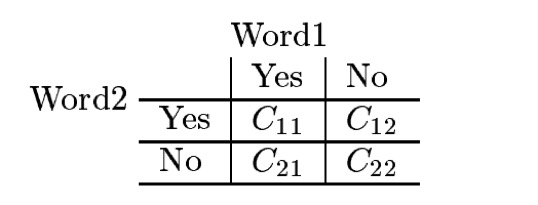
\includegraphics[width = 0.4\linewidth]{./FIG/030/contigency}\hfill
\label{fig:020feature}
\end{figure*}
For each word pair, $C_{11}$ is the count of sentences in the training corpus that contains the word pair; $C_{12}$ is the 
subtraction of the count of sentences contains word1 and $C_{11}$; $C_{21}$ is the subtraction of the count of sentences contains word2 and $C_{11}$; $C_{22}$ is the total number of sentences subtracting $C_{11}$, $C_{12}$ and $C_{21}$.\\
\\Then we calculate the Q-statistics as the correlation value between word pairs:
\begin{equation}
	Q=\frac{C_{11}C_{22} - C_{12}C_{21}}{C_{11}C_{22} + C_{12}C_{21}}
\end{equation}
The higher value of Q, the stronger the correlation between the two words.\\\\
Based on the above two categories, we designed our features as:
\vspace{-\topsep}
\begin{itemize}
  \setlength{\itemsep}{4pt}
    \setlength{\parskip}{0pt}
%    \setlength{\parsep}{0pt}  
  \item The ratio of stop words and content words.
  \item The general statistics of correlation value of word pairs.\\[5pt]
We calculate the mean, variance, maximum, minimum, mean and range of the correlation value of word pairs. Moreover, we created a subgroup of words pairs that only contains distant word pairs (distance  $\geq$5) and calculated the above feature for this group too.
 \item Percentage of high correlation values.\\[5pt]
This features detects the percentage of pairs that have high correlation values. We use a threshold to determine what is the standard of high.
 \item Percentage of unseen pairs.\\[5pt]
Real articles would have a relative stable percentage of unseen pairs while fake articles will have either too high or too low percentage. We believe that this feature can help us distinguish between real and fake.
 \item Repetition of phrases.\\[5pt]
Similar to the previous one, real articles would have a relative stable percentage of phrases repetitions while fake articles will have either too much repetition or little repetitions. We calculate the percentage of repetitions and the length of longest repeated phrases (single words are treated as special phrases too).
 \item Coherence score.\\[5pt]
Coherence score are defined as the average correlation value of distant (distance $\geq$5) content pairs.
 \item Latent Semantic Analysis (LSA).\\[5pt]
Inspired by the indexing technology, we've applied the idea of LSA to create a new feature which we believe can help improving the classification performance.[2] Let $X_{m\times{n}}$ be a matrix where element $X_{ij}$ describes the frequency of $Word_{i}$ in $Sentence_{j}$. Now, the dot product of $A_{n\times{n}} = X^{T}X$ contains all the dot products between the word vectors gives the correlation between the term over sentences. By using singular value decomposition (SVD), we can get  \begin{equation}
	A = U\Sigma{V^T}	
\end{equation}
Here, $\Sigma_{n\times{n}}$ is the diagonal matrix contains the singular value. Based on LSA, when you select the top $k$ largest singular values and their corresponding singular vectors from $U$ and $V$, you get the approximation to $A$. We use a threshold to select the top $k$ singular values and calculate the $A_{k}$. We use
\begin{equation}
	loss = \|A - A_{k}\|
\end{equation}
as the feature which represent the information loss using approximation. For real articles, the loss should be small while fake articles should be relatively large.

 
\end{itemize}


\subsection{Syntactic Feature}
Based on the hypothesis that trigram model cannot capture the syntactic features of sentence and the fake sentence are less grammatical, we measures the grammaticality of a sentence and uses it as one of our feature. More precisely, we parsed both real and fake sentences in the training data using the Charniak Parser in NLTK and got the likelihood of the highest ranked parsing tree for each sentence. We derived the overall grammaticality score by 
$$P_{Gram} = \frac{\sum_{i=1}^N L_iP(S_i)}{\sum_{i=1}^N L_i}$$
However, the syntactic feature is only able to improve the prediction a little bit in the training set and is very time-consuming. Thus, we abandoned it to be further used in the test set.
The potential reason for the syntactic feature to be such useless might be that our data contains spoken scripts, which are much less grammatical than the official written language. Another reason might be that the parser is not accurate, since it was trained in mixcase corpus, while our corpus was all uppercase.

\subsection{Statistical Feature}
Since the trigram model cannot capture information in the quad-gram model, we uses the ratio of perplexity of trigram and quad-gram models as one of the features. Since our training data is very small, the variance of the estimation will be very big. Thus, we used the same BNC corpus to estimate the probabilities of both trigram and quad-gram models. While the two type of articles will both have low perplexity score for the tri-gram model, the real articles would have lower perplexity for the quad-gram model than the fake articles. This implies that the ratio of trigram to quad-gram perplexities would be lower for a fake article than for a real article. Figure \ref{fig:ratio} shows the distribution of the feature in real articles and fake articles in the training data. As we can see, there is a significant difference of the feature between real and fake articles, which indicates that this is a good feature for distinguish two types of articles. 

\begin{figure*}
\centering  
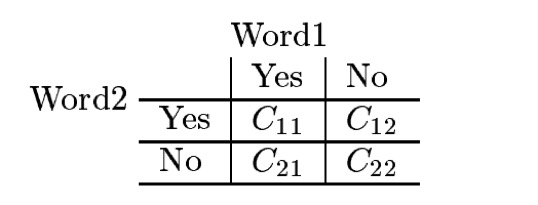
\includegraphics[width = 0.4\linewidth]{./FIG/030/ratio}\hfill
\caption{Histogram for the ratio of perplexity of trigram and quadgram} label{fig:ratio}
\end{figure*}

